\section{Research Inspiration}


\subsection{Vase or Face?}


Rubin, a Danish psychologist and philosopher, generated a well-known
ambiguous image, as shown in Fig.~\ref{fig:rubin_vase}, and first
introduced it in his doctoral thesis in 1915
\cite{rubin1915synsoplevede}. Rubin's vase is an example of the
cognitive optical illusion, which presents the viewer with a mental
choice of two valid shape interpretations. One interpretation is two
opposite black faces in the foreground with a white background. The
other one is a white vase in the foreground with a black
background. Generally, only one interpretation can be maintained at a
given moment, and the viewer will realize the second one after some
time or prompting. Thus, it is impossible to perceive both
interpretations simultaneously since one occludes the other.


   \begin{figure}
      \centering
      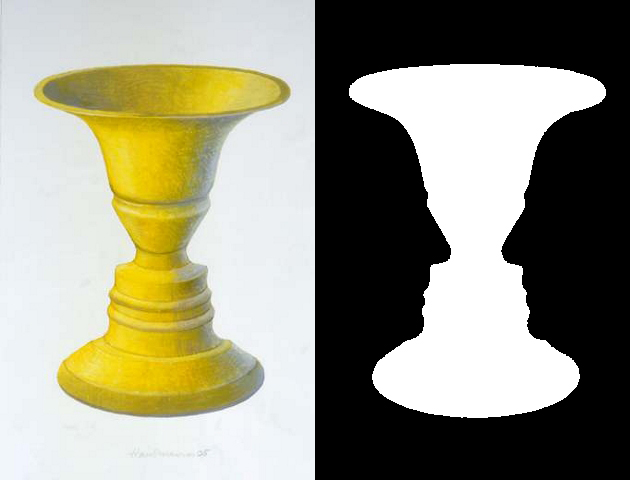
\includegraphics[width=\textwidth]{Rubin.png}
      \caption{From the left subfigure, some people may only see a
        symmetrical vase. However, if we look at the vase's right or
        left edge and consider the innermost indent as the tip of the
        nose outline, the indent above as the eye outline, and the
        double indent below as the mouth outline, people will see two
        opposite faces as shown in the right black-and-white
        subfigure.}
      \label{fig:rubin_vase}
   \end{figure}


Rubin has explained the illusion, which demonstrated how the brain
makes the figure-ground distinction during visual perception. In a
picture, if one object surrounds another, the surrounded object can be
considered as a figure, and the other object can be regarded as the
ground, and vice versa. If the figure and ground have a common border,
the ambiguity begins to creep in, and the brain can interpret the
black area as a figure or ground. Rubin's figure-ground distinction
has a profound impact on the psychologists to discover more similar
illusions \cite{mather2006foundations} and intrigue some artists to
construct objects in a reversion fashion \cite{bool1982mc}.


From Rubin's vase ambiguous image, we can detect two quite distinct
shapes, i.e. vase and faces, by having the perspectival switch and
paying attention to the figure and ground, respectively. Therefore,
the meaning and information of an image are stored in both foreground
and background. However, people are only concentrated on the figure
(i.e. plant roots with white pixels) and not the ground
(i.e. unoccupied space with black pixels) since all existing
descriptors are designed to characterize the plant roots in $2
$dimensional images. In this case, unlike the application of Rubin's
vase in neural analysis, psychology, art, and so on, we aim to explore
the unoccupied space for understanding plant root images.




\subsection{Kac’s Idea: Can One Hear the Shape of a Drum? \cite{kac1966can}}



  \subsubsection{Interpretations of Kac's Problem}

     \begin{itemize}
       \item When the drum vibrates, one can hear the sound, which is composed of tones of various frequencies. How much can shape features be inferred from hearing a discrete spectrum of pure tones produced by a drum?
       \item If a complete sequence of eigenvalues of the Dirichlet problem for the Laplacian can be obtained precisely, will people determine the shape of a planar?
     \end{itemize}




    \subsubsection{Problem Statement}

     \begin{itemize}     
       \item Consider a simply connected membrane $\Omega$ in the Euclidean space bounded by a smooth convex curve $\partial \Omega$ (e.g. a drum without any holes)
       \item Find function $\phi$ on the closure of $\Omega$, which vanishes at the boundary $\partial \Omega$, and a number $\lambda$ satisfying $-\Delta \phi = \lambda \phi$.

         \begin{itemize}
           \item $\Delta$ is the Laplace operator. e.g. $\Delta = \sum_{i=1}^{n} \frac{\partial ^2}{\partial x_i^2}$ in Cartesian coordinate system.
           \item If there exists a solution $\phi \neq 0$, the corresponding $\lambda$ is defined as a Dirichlet eigenvalue.
           \item For each domain $\Omega$, there has a sequence of eigenvalues $\lambda_1, \lambda_2, \lambda_3, ... $ corresponding to a set of eigenfunction $\phi_1, \phi_2, \phi_3, ...$.
           \item $\phi_k$ form an orthonormal basis of $L^2(\Omega)$ of real valued eigenfunctions; the corresponding discrete Dirichlet eigenvalues are positive ($\lambda_k \in \mathbb{R}^{+}$).
         \end{itemize}
         
       \item An important function \cite{grieser2013hearing}:

         \begin{equation}\label{eq:heat_trace}
           h(t) = \sum_{k=1}^{\infty} e^{-\lambda_kt}
         \end{equation}
         
         \begin{itemize}  
           \item It is a Dirichlet series.
           \item It is called the spectral function or the heat trace.
           \item It is smooth and converges for every $t>0$.
         \end{itemize}
     \end{itemize}



     \subsubsection{Summarize the Results of Kac's Idea}

       \begin{equation}\label{eq:kac_result}
          h(t) = \sum_{k=1}^{\infty} e^{-\lambda_kt} \sim \frac{|\Omega|}{2\pi t} - \frac{L}{4} \frac{1}{\sqrt{2\pi t}} + \frac{1}{6}
       \end{equation}
     
      \begin{itemize} 
        \item As $t \rightarrow 0^{+}$, the leading terms of the asymptotic expansion of $h(t)$ imply the geometrical attributes of $\Omega$
          \begin{itemize}
            \item the total area
            \item the perimeter
            \item the curvature
          \end{itemize}
          
        \item If the domain $\Omega$ has the polygonal boundary, the third term shows in the information about the interior angles of the polygon \cite{grieser2013hearing}.
      \end{itemize}



    \subsubsection{Conclusion}

     \subsubsubsection{Advantages}

        \begin{itemize}
          \item Kac proposed a novel analytical mathematical method for the shape description without using measuring tools, e.g. rulers.
          \item Other mathematicians extended Kac's idea in exploring the geometrical information of more complex domains with various boundary conditions \cite{khabou2007shape}\cite{gottlieb1985eigenvalues}\cite{gottlieb1983hearing} \cite{zayed1989heat}\cite{sleeman1984trace}.
        \end{itemize}
        
     \subsubsubsection{Limitations}
        
        \begin{itemize}
          \item It is only available for the convex domain, which has a smooth or piecewise smooth boundary.  
          \item Except in very few cases (i.e. rectangular, disk, certain triangles), the complete sequence of eigenvalues $\lambda_k$ can not be calculated \cite{grieser2013hearing}.
          \item Only the first few terms in the asymptotic expansion of $h(t)$ are explicitly available.
        \end{itemize}


        



\subsection{Extended Work of Kac’s Idea: Heat Content $Q(\tau)$ \cite{vandenberg1994heat}}



  \subsubsection{Fouier's Heat Equation \cite{baron1878analytical}}

  \begin{itemize}
    \item Mathematical Formula
        \par
        \begin{equation}\label{eq:heat_equation}
          \frac{\partial u(\bm{s}, t)}{\partial t} = \Delta u(\bm{s}, t)
        \end{equation}

   \item Interpretation
     \par
     It is a deterministic model used to characterize the evolution of quantities over the space and time. (e.g. the flow of heat)
  \end{itemize}




  \subsubsection{Summarize the Idea}

   \begin{itemize}
      \item Initial-Boundary Value Problem (IBVP)
        \par
        $u(\bm{s}, t)$ indicates the value of the tempretature at $\bm{s} \in \Omega$ at time $t$ satisfying Eq.~\ref{eq:heat_equation} and
        \begin{itemize}
          \item Initial condition: $u(\bm{s}, t) = f(\bm{s})$ as $t \rightarrow 0$.
          \item Dirichlet boundary condition: $u(\bm{s}, t)=0$ for $\bm{s} \in \partial \Omega$
            \par
            It is also called the absorbing boundary condition; i.e. any molecule will be instantly absorbed when it touches the boundary $\partial \Omega$;
        \end{itemize}

      \item A Basic Integration

        \par
          \begin{align}
            \beta_{\Omega}(f, g)(t) &= \int_{\Omega} \int_{\Omega} H_{\Omega}(\bm{s}, t | \bm{s_0}) f(\bm{s_0}) g(\bm{s}) d\bm{s_0} d\bm{s} \label{eq:integral_full} \\
            &= \int_{\Omega} u(\bm{s}, t) g(\bm{s}) d\bm{s} \label{eq:integral_convol}
          \end{align}


        \begin{itemize}
           \item $H_{\Omega}(\bm{s}, t | \bm{s_0})$ is called the heat kernel of $\Omega$ describing the density of the heat at $\bm{s}$ after time $t$ when initially there is only one single hot source at $\bm{s_0}$.
           \item $u(\bm{s}, t)$ is the general solution to Eq.~\ref{eq:heat_equation}, which can be expressed as the convolution of the initial condition with the heat kernel of the domain.
           \item $g(\bm{s})$ is an auxiliary test function for studying the distributional nature of the tempretature function $u(\bm{s}, t)$ near $\partial \Omega$.
        \end{itemize}


      \item Heat Content Calculation

        \par
       Given 
       \begin{equation} \label{eq:g}
         g(\bm{s}) = 1  
       \end{equation}

       \begin{align}
         Q_{\Omega}(t) &= \int_{\Omega} \int_{\Omega} H_{\Omega}(\bm{s}, t | \bm{s_0}) f(\bm{s_0})  d\bm{s_0} d\bm{s} \label{eq:heat_content_integral_full} \\
            &= \int_{\Omega} u(\bm{s}, t) d\bm{s} \label{eq:heat_content_integral_convol}
       \end{align}


     \item Shape Characterization

       \begin{itemize}
       \item As $t \rightarrow 0^{+}$,

         \begin{equation}\label{eq:heat_content_asy}
           Q_{\Omega}(t) \simeq \sum_{n=1}^{\infty} \beta_n(\Omega) t ^{\frac{n}{2}}
         \end{equation}
         
         
         \item Obtain geometrical information of $\Omega$ from $\beta_n$
           \begin{itemize}
           \item area
           \item length
           \item scalar curvature
           \item mass
         \end{itemize}
       \end{itemize}
       
       
   \end{itemize}



  \subsubsection{Conclusion}

    \begin{itemize}
      \item Strengthness
        \begin{itemize}
          \item Instead of calculating a complete sequence of the Dirichlet eigenvalues for exploring the shape attributes of geometry, the asymptotic expansion of the heat content, defined as integrating the solution to the heat equation over the space-dimension, also implies the geometrical characteristics.  
        \end{itemize}
        
      \item
        \begin{itemize}
          \item Only the infinitly differentiable boundary $\partial \Omega$ is considered.
          \item Only the first few terms in the asymptotic expansion are explicitly known.
          \item Either irregular geometries or discontinuities lead to the complexities, so the explicit solutions $u(\bm{s}, t)$ are close to non-existed.
          \item The numerical evaluation of the analytical $u(\bm{s}, t)$ and $Q_{\Omega}(t)$ is usually by no means trivial because they are in the form of infinite series.
          \item Similiarly, only the first few coeffients $\beta_n$ in the asymptotic expansion of $Q_{\Omega}(t)$ can be expressed as the complicated explicit forms.
        \end{itemize}
        
    \end{itemize}
    




In this section, we have a perceptual shift and begin understanding
the plant root images from a reversing view, that is, to explore and
distinguish the unoccupied space in the image, i.e. the region without
roots, to reveal and compare both geometric and spatial attributes of
plant roots. Also, we are intrigued by Kac's idea about using
analytical mathematical tools for shape characterization to overcome
the limitations of conventional ruler-based measurements. The heat
content calculation is an extension of Kac's idea, which presents a
relatively practicable mathematical method to describe an irregular
compact region with a smooth boundary. However, it is still
challenging and time-consuming to solve the initial-boundary value
problem by either analytical or numerical methods.
